\newpage
\section{遊泳実験}
外皮の有無による遊泳性能への影響を検証するために,胴体外皮未装着時と胴体外皮装着時それぞれで直進遊泳実験を行った.図\ref{fig:doutainasi}に胴体外皮未装着時の状態を示す.

\subsection{実験条件}
サーボモータには昨年度卒業研究と同様にステップ上の入力を与えた(図\ref{fig:servo_seigyo}).$T$ [ms]は入力の周期,$\theta$ [deg]はプーリの回転角(糸の巻き取り量)を表してい
る.ここでこの実験で使用する尾びれ周波数と尾びれ振幅という二つのパラメータをついて述べる.まず尾びれ周波数は尾びれを振る速さを決定するパラメータであり,$f = 1/T$ [Hz]で算出する.
尾びれ振幅は体をどのくらい屈曲させるかのパラメータであり,トラッキングソフト「kinovea」を用いて尾びれの振れ角を算出し,それを尾びれ振幅とした(図\ref{fig:obire_amp}). 

直進遊泳実験は尾びれ振幅を一定にし,尾びれ周波数を変更した時の速度を測定した.尾びれ振幅はプーリの回転角を$30\:^\circ$,$45\:^\circ$,$60\:^\circ$としたときのそれぞれのトラッ
キング角度$81\:^\circ$,$114\:^\circ$,$168\:^\circ$で一定にし,尾びれ周波数は0.5~1.75 Hzまで0.25 Hzずつ変化させ,合計54 個のパラメータについて実験を行った.
各パラメータにつき3回実験を行い,得られた遊泳速度のデータから平均,分散,標準偏差を算出した.
\begin{figure}[htbp]
    \centering
    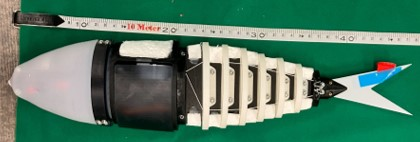
\includegraphics[width=0.8\linewidth]{chapters/picture/without_skin.jpg}
    \caption{胴体外皮未装着の状態}
    \label{fig:doutainasi}
\end{figure}
\begin{figure}[htbp]
    \centering
     \begin{minipage}[b]{0.5\linewidth}
        \centering
        \setPicture{servo.png}
        \caption{サーボへの制御入力}
        \label{fig:servo_seigyo}
     \end{minipage}
     \hspace{0.05\linewidth}
     \begin{minipage}[b]{0.4\linewidth}
        \centering
        \setPicture{obire_amp.png}
        \caption{尾びれ振幅について}
        \label{fig:obire_amp}
     \end{minipage}
\end{figure}
次に遊泳速度の算出方法について述べる.まずは天井に取り付けたカメラを用いて撮影した動画から尾びれに取り付けたマーカーをkinoveaでトラッキングする.そして得られた尾びれ軌跡のトラッキングデータ
を二次近似し,積分して遊泳距離を算出し,遊泳時間で除算して遊泳速度を算出する.直進遊泳開始時に過渡状態となることを踏まえ,トラッキング範囲を遊泳を開始してから500~1500 mmの範囲に設定した.

\subsection{実験結果}
図に振幅,周波数の時の遊泳実験の様子を,図に実験結果を示す.図のエラーバーは算出した標準偏差を示している.遊泳実験では,すべてのパラメータで直進させたかったが,何回か進行方向が右に傾いたり左
に傾いたりしてしまう時があった.図から,まず外皮あり・なし両方に共通して周波数が高くなるほど


